\documentclass{standalone}
\usepackage{graphicx}
\usepackage{tikz}
% Tikz libraries
\usetikzlibrary{%
    patterns, plotmarks, backgrounds, shapes, arrows, calc, trees, positioning,
    chains, shapes.geometric, decorations.pathreplacing,
    decorations.pathmorphing, shapes.arrows, decorations.markings, quotes, 
    shapes.geometric, arrows.meta, spy, fit, matrix, math, bending, graphs,
    graphs.standard, through
}

\usepackage{xcolor}
\usepackage{caption}
\usepackage{subcaption}
\captionsetup{justification=raggedright,singlelinecheck=false}
\usepackage{chemfig}
\usepackage{amsmath}

% Define colours
\definecolor{cred}{HTML}{ED1C24}
\definecolor{cgrey}{HTML}{7F7F7F}
\definecolor{cblue}{HTML}{00A2E8}
\definecolor{cgreen}{HTML}{22B14C}
\definecolor{cyellow}{HTML}{FFF200}
\definecolor{corange}{HTML}{EA7904}
\definecolor{cpurple}{HTML}{9100FC}

\usepackage[most]{tcolorbox}
\tcbset{%
    on line,
    boxsep=4pt, left=0pt,right=0pt,top=0pt,bottom=0pt,
    arc=7.5pt,
    colframe=white,
    %colback=LightLavender,
    highlight math style={enhanced}
}
\renewcommand{\familydefault}{\sfdefault}

\setchemfig{%
    scheme debug=false,
    atom style={scale=0.5},
    atom sep=2em,
    bond offset=1pt
}

\begin{document}

\begin{figure}
    \begin{subfigure}[t]{1.43\textwidth}
        \caption{}
        \begin{tikzpicture}
            \node (G6P)
                []
                {%
                    \chemfig{%
                                  OH% 8
                         -[:90,,1]% 6
                           %-[:150]% 5
                           -[:150]{\colorbox{corange}{\color{black}{C}}}
                                     (%
                           -[:210,,,2]HO% 9
                                     )
                            %-[:90]% 4
                            -[:90]{\colorbox{cblue}{\color{black}{C}}}
                                     (%
                           -[:150,,,2]HO% 10
                                     )
                            %-[:30]% 3
                            -[:30]{\tcbox[colback=cblue]{C}}
                                     (%
                            -[:90,,,1]OH% 11
                                     )
                           %-[:330]% 2
                           -[:330]{\tcbox[colback=corange]{C}}
                                     (%
                               -[:270]O% 7
                               %-[:210]% -> 6
                               -[:210]{\colorbox{cgreen}{\color{black}{C}}}
                                     )
                            %-[:30]% 1
                            -[:30]{\tcbox[colback=cgreen]{C}}
                           -[:330]O% 12
                            -[:30]P% 13
                                     (%
                                =[:90]O% 14
                                     )
                                     (%
                           -[:330,,,1]OH% 15
                                     )
                        -[:30,,,1]OH% 16
                    }
                };
              \node[below=0.1cm of G6P] () {G6P};
              \node (arr1)
                [right=0.1cm of G6P]
                {\schemestart\arrow{<=>}\schemestop};
              \node (F6P)
                [right=0.1cm of arr1]
                {%
                  \chemfig{%
                                 O% 6
                           %=[:90]% 5
                           =[:90]{\colorbox{corange}{\color{black}{C}}}
                                    (%
                              %-[:150]% 7
                              -[:150]{\colorbox{cgreen}{\color{black}{C}}}
                          -[:210,,,2]HO% 8
                                    )
                           %-[:30]% 4
                           -[:30]{\colorbox{cblue}{\color{black}{C}}}
                                    (%
                           -[:90,,,1]OH% 9
                                    )
                          %-[:330]% 3
                          -[:330]{\tcbox[colback=cblue]{C}}
                                    (%
                          -[:270,,,1]OH% 10
                                    )
                           %-[:30]% 2
                           -[:30]{\tcbox[colback=corange]{C}}
                                    (%
                           -[:90,,,1]OH% 11
                                    )
                          %-[:330]% 1
                          -[:330]{\tcbox[colback=cgreen]{C}}
                           -[:30]O% 12
                          -[:330]P% 13
                                    (%
                              =[:270]O% 14
                                    )
                                    (%
                           -[:30,,,1]OH% 15
                                    )
                      -[:330,,,1]OH% 16
                  }
                };
              \node[below=0.1cm of F6P] () {F6P};
              \node (arr2)
                [right=0.1cm of F6P]
                {\schemestart\arrow{-U>[\tiny ATP][\tiny ADP][][0.25]}\schemestop};
              \node (F16P)
                [right=0.1cm of arr2]
                {%
                  \chemfig{%
                               O% 10
                        =[:228]P% 9
                                  (%
                        -[:168,,,2]HO% 11
                                  )
                                  (%
                        -[:108,,,2]HO% 12
                                  )
                        -[:288]O% 8
                        %-[:348]% 7
                        -[:348]{\tcbox[colback=cgreen]{C}}
                        %-[:288]% 5
                        -[:288]{\tcbox[colback=corange]{C}}
                                  (%
                        -[:192,,,2]HO% 13
                                  )
                        %-[:276]% 4
                        -[:276]{\tcbox[colback=cblue]{C}}
                                  (%
                        -[:222,,,2]HO% 14
                                  )
                        %-[:348]% 3
                        -[:348]{\colorbox{cblue}{\color{black}{C}}}
                                  (%
                        -[:294,,,1]OH% 15
                                  )
                         %-[:60]% 2
                         -[:60]{\colorbox{corange}{\color{black}{C}}}
                                  (%
                            -[:132]O% 6
                            -[:204]{\tcbox[colback=corange]{C}}% -> 5
                                  )
                          %-[:6]% 1
                          -[:6]{\colorbox{cgreen}{\color{black}{C}}}
                         -[:66]O% 16
                          -[:6]P% 17
                                  (%
                            =[:306]O% 18
                                  )
                                  (%
                         -[:66,,,1]OH% 19
                                  )
                      -[:6,,,1]OH% 20
                  }
                };
              \node[below=0.1cm of F16P] () {FDP};

              \node (G3P)
                [right=1.0cm of F16P, yshift=1.25cm]
                {%
                  \chemfig{%
                                O% 4
                          %=[:30]% 3
                          =[:30]{\colorbox{cblue}{\color{black}{C}}}
                         %-[:330]% 2
                         -[:330]{\colorbox{corange}{\color{black}{C}}}
                                   (%
                         -[:270,,,1]OH% 5
                                   )
                          %-[:30]% 1
                          -[:30]{\colorbox{cgreen}{\color{black}{C}}}
                         -[:330]O% 6
                          -[:30]P% 7
                                   (%
                             =[:330]O% 8
                                   )
                                   (%
                          -[:90,,,1]OH% 9
                                   )
                      -[:30,,,1]OH% 10
                  }
                };
              \node[above=0.1cm of G3P] () {G3P};
              \node (DHAP)
                [right=1.0cm of F16P, yshift=-1.25cm]
                {%
                  \chemfig{%
                               O% 3
                         %=[:90]% 2
                         %=[:90]{\colorbox{corange}{\color{black}{C}}}
                         =[:90]{\tcbox[colback=corange]{C}}
                                  (%
                             %-[:30]% 1
                             %-[:30]{\colorbox{cblue}{\color{black}{C}}}
                             -[:30]{\tcbox[colback=cblue]{C}}
                        -[:330,,,1]OH% 10
                                  )
                        %-[:150]% 4
                        %-[:150]{\colorbox{cgreen}{\color{black}{C}}}
                        -[:150]{\tcbox[colback=cgreen]{C}}
                        -[:210]O% 5
                        -[:150]P% 6
                                  (%
                            =[:210]O% 7
                                  )
                                  (%
                         -[:90,,,1]OH% 8
                                  )
                    -[:150,,,2]HO% 9
                }
              };
              \node[below=0.1cm of DHAP] () {DHAP};

              \node (arr3) at ($(G3P)!0.5!(DHAP)$)
                [rotate=90]
                {\schemestart\arrow{<=>}\schemestop};
              \draw[-stealth] (F16P) -- ( $ (F16P.0)!0.5!(G3P.west|-F16P.0) $ ) |- (G3P.west) node[auto,pos=0.7] {};
              \draw[-stealth] (F16P) -- ( $ (F16P.0)!0.5!(DHAP.west|-F16P.0) $ ) |- (DHAP.west) node[auto,pos=0.7] {};
        \end{tikzpicture}
        \caption{}
        \begin{tikzpicture}
            \node (glut1)
                []
                {
            \chemfig{%
                           O% 4
                     =[:90]% 3
                              (%
                         -[:30]% 2
                         -[:330]{\colorbox{cblue}{\color{black}{C}}}% 1
                         -[:30]% 16
                                  (%
                         -[:90,,,1]NH_2% 20
                                  )
                        -[:330]% 17
                                  (%
                         -[:30,,,1]OH% 19
                                  )
                        =[:270]O% 18
                              )
                    -[:150]\mcfabove{N}{H}% 5
                    -[:210]% 6
                              (%
                        -[:270]% 7
                    -[:330,,,1]SH% 8
                              )
                    -[:150]% 9
                              (%
                         =[:90]O% 10
                              )
                    -[:210]\mcfbelow{N}{H}% 11
                    -[:150]% 12
                    -[:210]% 13
                              (%
                        =[:270]O% 14
                              )
                -[:150,,,2]HO% 15
            }
                };
                \node[below=0.1cm of glut1] () {Glutathione};

                \node (p1)
                    [below=1.0cm of glut1]
                    {
                \schemestart\ \+ \schemestop
                    };
            \node (glut2)
                [below=0.1cm of p1]
                {
            \chemfig{%
                           O% 4
                     =[:90]% 3
                              (%
                         -[:30]% 2
                         -[:330]{\colorbox{corange}{\color{black}{C}}}% 1
                         -[:30]% 16
                                  (%
                         -[:90,,,1]NH_2% 20
                                  )
                        -[:330]% 17
                                  (%
                         -[:30,,,1]OH% 19
                                  )
                        =[:270]O% 18
                              )
                    -[:150]\mcfabove{N}{H}% 5
                    -[:210]% 6
                              (%
                        -[:270]% 7
                    -[:330,,,1]SH% 8
                              )
                    -[:150]% 9
                              (%
                         =[:90]O% 10
                              )
                    -[:210]\mcfbelow{N}{H}% 11
                    -[:150]% 12
                    -[:210]% 13
                              (%
                        =[:270]O% 14
                              )
                -[:150,,,2]HO% 15
            }
                };
            \node[below=0.1cm of glut2] () {Glutathione};
                \node (p1B)
                    [below=1.0cm of glut2]
                    {
                \schemestart\ \+ \schemestop
                    };

            \node (h2o2)
                [below=0.1cm of p1B]
                {
                  \chemfig{%
                              HO% 1
                      -[,,2,1]OH% 2
                    }
                };

            \node (arr1)
            [right=2.1cm of p1]
            {
                \schemestart\ \arrow{<=>[Glutathione peroxidase][(Mitochondria)]}[0, 2.5]\schemestop\
            };

            \node (glutdi)
                [right=0.1cm of arr1]
                {
            \chemfig{%
                           O% 4
                    =[:270]% 3
                              (%
                        -[:330]% 2
                         -[:30]{\colorbox{corange}{\color{black}{C}}}% 1
                        -[:330]% 36
                                  (%
                        -[:270,,,1]NH_2% 40
                                  )
                         -[:30]% 37
                                  (%
                        -[:330,,,1]OH% 39
                                  )
                         =[:90]O% 38
                              )
                    -[:210]\mcfbelow{N}{H}% 5
                    -[:150]% 6
                              (%
                        -[:210]% 29
                                  (%
                            -[:150]\mcfabove{N}{H}% 31
                            -[:210]% 32
                            -[:150]% 33
                                      (%
                            -[:210,,,2]HO% 35
                                      )
                             =[:90]O% 34
                                  )
                        =[:270]O% 30
                              )
                     -[:90]% 7
                     -[:30]S% 8
                     -[:90]S% 9
                     -[:30]% 10
                     -[:90]% 11
                              (%
                         -[:30]% 12
                                  (%
                         -[:90,,,2]HN% 14
                          -[:30,,2]% 15
                             -[:90]% 16
                                      (%
                             -[:30,,,1]OH% 18
                                      )
                            =[:150]O% 17
                                  )
                        =[:330]O% 13
                              )
                -[:150,,,2]HN% 19
                  -[:90,,2]% 20
                              (%
                         =[:30]O% 21
                              )
                    -[:150]{\colorbox{cblue}{\color{black}{C}}}% 22
                     -[:90]% 23
                    -[:150]% 24
                              (%
                    -[:210,,,2]H_2N% 28
                              )
                     -[:90]% 25
                              (%
                         =[:30]O% 26
                              )
                -[:150,,,2]HO% 27
            }
                };
                \node[below=0.1cm of glutdi] () {Glutathione disulfide};

                \node (p2)
                    [right=0.1cm of glutdi]
                    {
                \schemestart\ \+ \schemestop
                    };
                \node (h2o)
                    [right=0.1cm of p2]
                    {
                      \chemfig{%
                          H_2O% 1
                      }
                    };

                \node (p3)
                    [right=0.1cm of h2o]
                    {
                \schemestart\ \+ \schemestop
                    };
                \node (h2oB)
                    [right=0.1cm of p3]
                    {
                      \chemfig{%
                          H_2O% 1
                      }
                    };
        \end{tikzpicture}
        \caption{}
        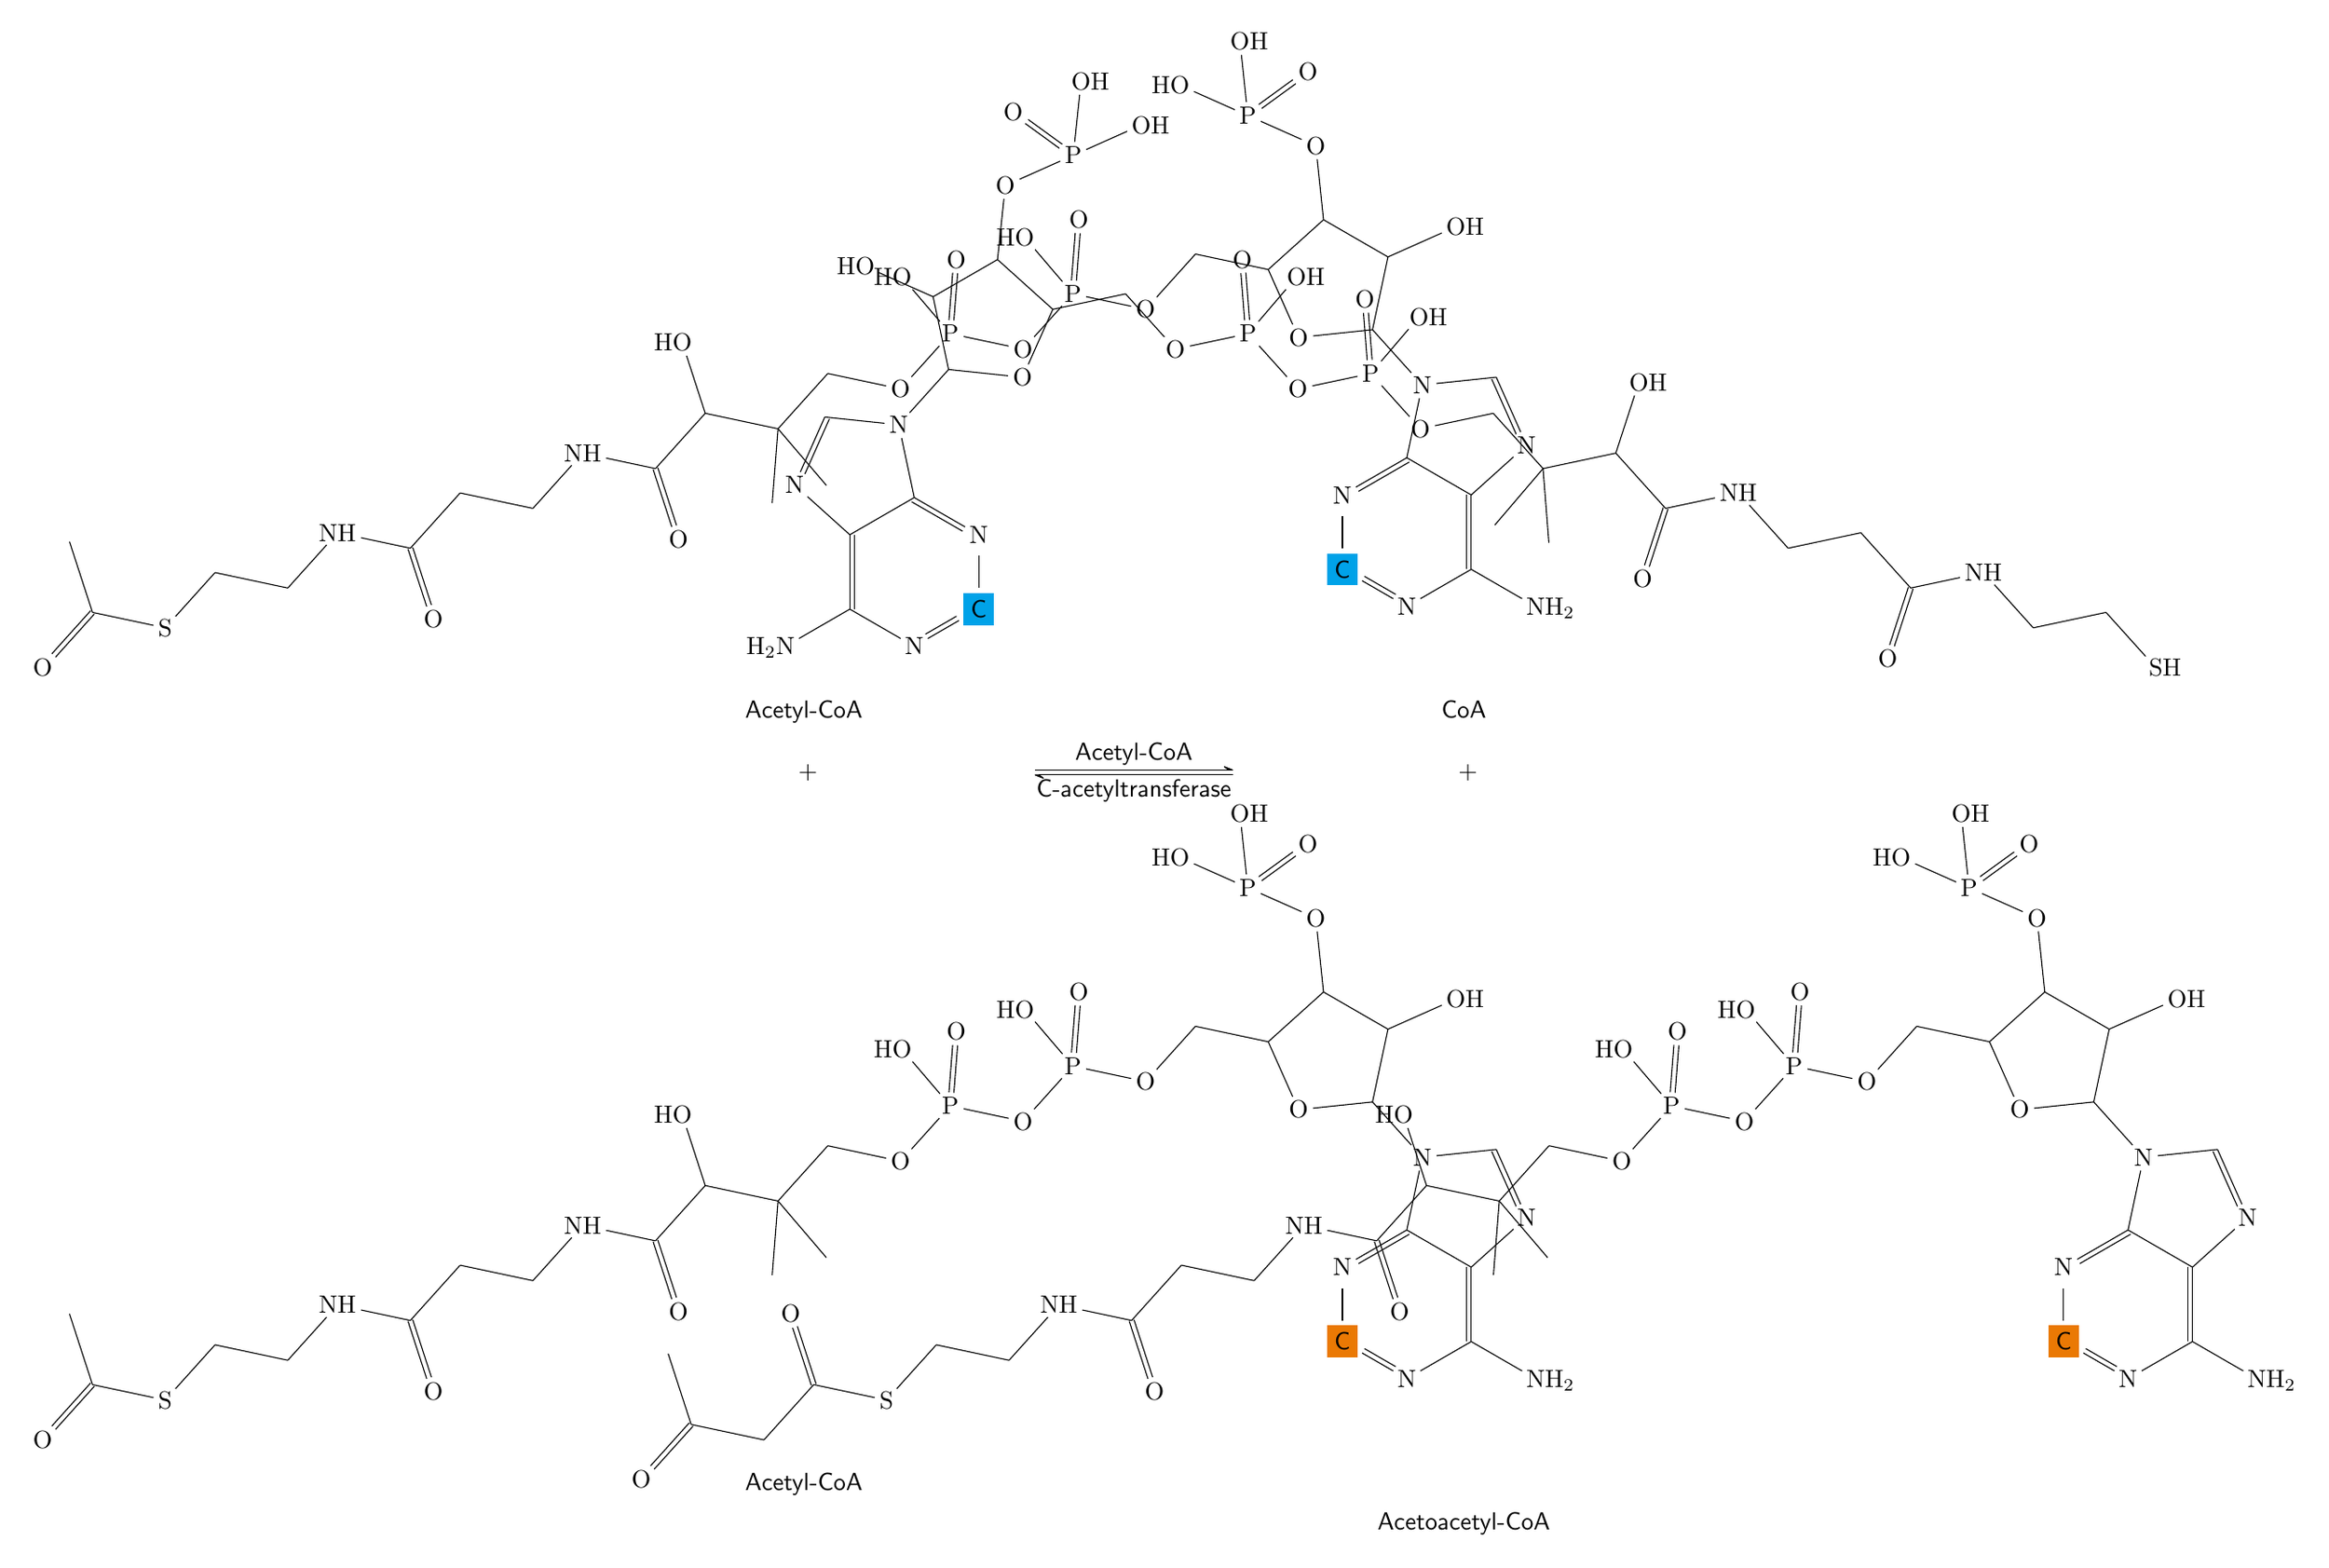
\begin{tikzpicture}
            \node (acoa1)
                []
                {
    \chemfig{% Acetyl-CoA
                 % 1
          -[:288]% 2
                    (%
              =[:228]O% 3
                    )
          -[:348]S% 4
           -[:48]% 5
          -[:348]% 6
           -[:48]\mcfabove{N}{H}% 7
          -[:348]% 8
                    (%
              =[:288]O% 9
                    )
           -[:48]% 10
          -[:348]% 11
           -[:48]\mcfabove{N}{H}% 12
          -[:348]% 13
                    (%
              =[:288]O% 14
                    )
           -[:48]% 15
                    (%
          -[:108,,,2]HO% 51
                    )
          -[:348]% 16
                    (%
            -[:265.5]% 17
                    )
                    (%
            -[:310.5]% 18
                    )
           -[:48]% 19
          -[:348]O% 20
           -[:48]P% 21
                    (%
             =[:85.5]O% 22
                    )
                    (%
        -[:130.5,,,2]HO% 23
                    )
          -[:348]O% 24
           -[:48]P% 25
                    (%
             =[:85.5]O% 26
                    )
                    (%
        -[:130.5,,,2]HO% 27
                    )
          -[:348]O% 28
           -[:48]% 29
          -[:348]% 30
           -[:42]% 31
                    (%
               -[:96]O% 46
              -[:156]P% 47
                        (%
              -[:156,,,2]HO% 49
                        )
                        (%
               -[:96,,,1]OH% 50
                        )
               =[:36]O% 48
                    )
          -[:330]% 32
                    (%
           -[:24,,,1]OH% 45
                    )
          -[:258]% 33
                    (%
              -[:186]O% 34
              -[:114]% -> 30
                    )
          -[:312]N% 35
            -[:6]% 36
         =_[:294]N% 37
          -[:222]% 38
         =_[:270]% 39
                    (%
          -[:330,,,1]NH_2% 44
                    )
          -[:210]N% 40
         =_[:150]{\colorbox{cblue}{\color{black}C}}% 41
           -[:90]N% 42
          =_[:30]% 43
                    (%
              -[:330]% -> 38
                    )
                    (%
               -[:78]\phantom{N}% -> 35
                    )
    }
                };
                \node[below=0.1cm of acoa1] () {Acetyl-CoA};
                \node (p1)
                    [below=1.0cm of acoa1]
                    {
                \schemestart\ \+ \schemestop
                    };

            \node (acoa2)
                [below=0.1cm of p1]
                {
    \chemfig{% Acetyl-CoA
                 % 1
          -[:288]% 2
                    (%
              =[:228]O% 3
                    )
          -[:348]S% 4
           -[:48]% 5
          -[:348]% 6
           -[:48]\mcfabove{N}{H}% 7
          -[:348]% 8
                    (%
              =[:288]O% 9
                    )
           -[:48]% 10
          -[:348]% 11
           -[:48]\mcfabove{N}{H}% 12
          -[:348]% 13
                    (%
              =[:288]O% 14
                    )
           -[:48]% 15
                    (%
          -[:108,,,2]HO% 51
                    )
          -[:348]% 16
                    (%
            -[:265.5]% 17
                    )
                    (%
            -[:310.5]% 18
                    )
           -[:48]% 19
          -[:348]O% 20
           -[:48]P% 21
                    (%
             =[:85.5]O% 22
                    )
                    (%
        -[:130.5,,,2]HO% 23
                    )
          -[:348]O% 24
           -[:48]P% 25
                    (%
             =[:85.5]O% 26
                    )
                    (%
        -[:130.5,,,2]HO% 27
                    )
          -[:348]O% 28
           -[:48]% 29
          -[:348]% 30
           -[:42]% 31
                    (%
               -[:96]O% 46
              -[:156]P% 47
                        (%
              -[:156,,,2]HO% 49
                        )
                        (%
               -[:96,,,1]OH% 50
                        )
               =[:36]O% 48
                    )
          -[:330]% 32
                    (%
           -[:24,,,1]OH% 45
                    )
          -[:258]% 33
                    (%
              -[:186]O% 34
              -[:114]% -> 30
                    )
          -[:312]N% 35
            -[:6]% 36
         =_[:294]N% 37
          -[:222]% 38
         =_[:270]% 39
                    (%
          -[:330,,,1]NH_2% 44
                    )
          -[:210]N% 40
         =_[:150]{\colorbox{corange}{\color{black}C}}% 41
           -[:90]N% 42
          =_[:30]% 43
                    (%
              -[:330]% -> 38
                    )
                    (%
               -[:78]\phantom{N}% -> 35
                    )
    }
                };
            \node[below=0.1cm of acoa2] () {Acetyl-CoA};
              \node (arr1)
                [right=2.3cm of p1]
                {\schemestart\arrow{<=>[Acetyl-CoA][C-acetyltransferase]}[0, 2.0]\schemestop};
                \node (p2)
                    [right=2.3cm of arr1]
                    {
                \schemestart\ \+ \schemestop
                    };
            \node (coa)
                [above=1.0cm of p2]
                {
    \chemfig{% CoA
                % 1
        -[:94.5]% 2
                   (%
           -[:229.5]% 3
                   )
                   (%
              -[:12]% 36
                       (%
              -[:72,,,1]OH% 48
                       )
             -[:312]% 37
                       (%
                  -[:12]\mcfabove{N}{H}% 39
                 -[:312]% 40
                  -[:12]% 41
                 -[:312]% 42
                           (%
                      -[:12]\mcfabove{N}{H}% 44
                     -[:312]% 45
                      -[:12]% 46
                 -[:312,,,1]SH% 47
                           )
                 =[:252]O% 43
                       )
             =[:252]O% 38
                   )
         -[:132]% 4
         -[:192]O% 5
         -[:132]P% 6
                   (%
            =[:94.5]O% 7
                   )
                   (%
        -[:49.5,,,1]OH% 8
                   )
         -[:192]O% 9
         -[:132]P% 10
                   (%
            =[:94.5]O% 11
                   )
                   (%
        -[:49.5,,,1]OH% 12
                   )
         -[:192]O% 13
         -[:132]% 14
         -[:192]% 15
         -[:138]% 16
                   (%
              -[:84]O% 31
              -[:24]P% 32
                       (%
              -[:24,,,1]OH% 34
                       )
                       (%
              -[:84,,,1]OH% 35
                       )
             =[:144]O% 33
                   )
         -[:210]% 17
                   (%
         -[:156,,,2]HO% 30
                   )
         -[:282]% 18
                   (%
             -[:354]O% 19
              -[:66]% -> 15
                   )
         -[:228]N% 20
         -[:174]% 21
        =^[:246]N% 22
         -[:318]% 23
        =^[:270]% 24
                   (%
         -[:210,,,2]H_2N% 29
                   )
         -[:330]N% 25
        =^[:30]{\colorbox{cblue}{\color{black}C}}% 26
          -[:90]N% 27
        =^[:150]% 28
                   (%
             -[:210]% -> 23
                   )
                   (%
             -[:102]\phantom{N}% -> 20
                   )
    }
                };
                \node[below=0.1cm of coa] () {\phantom{y}CoA\phantom{y}};
            \node (aacoa)
                [below=0.1cm of p2]
                {
    \chemfig{% Acetoacetyl-CoA
                 % 1
          -[:288]% 2
                    (%
              =[:228]O% 3
                    )
          -[:348]% 4
           -[:48]% 5
                    (%
              =[:108]O% 6
                    )
          -[:348]S% 7
           -[:48]% 8
          -[:348]% 9
           -[:48]\mcfabove{N}{H}% 10
          -[:348]% 11
                    (%
              =[:288]O% 12
                    )
           -[:48]% 13
          -[:348]% 14
           -[:48]\mcfabove{N}{H}% 15
          -[:348]% 16
                    (%
              =[:288]O% 17
                    )
           -[:48]% 18
                    (%
          -[:108,,,2]HO% 54
                    )
          -[:348]% 19
                    (%
            -[:265.5]% 20
                    )
                    (%
            -[:310.5]% 21
                    )
           -[:48]% 22
          -[:348]O% 23
           -[:48]P% 24
                    (%
             =[:85.5]O% 25
                    )
                    (%
        -[:130.5,,,2]HO% 26
                    )
          -[:348]O% 27
           -[:48]P% 28
                    (%
             =[:85.5]O% 29
                    )
                    (%
        -[:130.5,,,2]HO% 30
                    )
          -[:348]O% 31
           -[:48]% 32
          -[:348]% 33
           -[:42]% 34
                    (%
               -[:96]O% 49
              -[:156]P% 50
                        (%
              -[:156,,,2]HO% 52
                        )
                        (%
               -[:96,,,1]OH% 53
                        )
               =[:36]O% 51
                    )
          -[:330]% 35
                    (%
           -[:24,,,1]OH% 48
                    )
          -[:258]% 36
                    (%
              -[:186]O% 37
              -[:114]% -> 33
                    )
          -[:312]N% 38
            -[:6]% 39
         =_[:294]N% 40
          -[:222]% 41
         =_[:270]% 42
                    (%
          -[:330,,,1]NH_2% 47
                    )
          -[:210]N% 43
          =_[:150]{\colorbox{corange}{\color{black}C}}% 44
           -[:90]N% 45
          =_[:30]% 46
                    (%
              -[:330]% -> 41
                    )
                    (%
               -[:78]\phantom{N}% -> 38
                    )
    }
                };
                \node[below=0.1cm of aacoa] () {Acetoacetyl-CoA};
        \end{tikzpicture}
    \end{subfigure}
\end{figure}

\end{document}
